\section{评估}
\label{sec:evaluation}

\subsection{协议}
\label{sec:protocol}

参考为 Mixbox~2.0 \texttt{lerpFloat} 的 sRGB 显示值浮点路径。度量为 CIEDE2000，取 $k_{L}=k_{C}=k_{H}=1$，按 \cref{sec:reference} 所述完成验证。随机集均值给出 bootstrap 95\% 置信区间（1000 次重采样，重采样流固定，故区间可复现）。$\Delta E_{00}$ 的感知刻度只作定性参考：小于 1 接近可察觉阈值，1--2 细看可见，2--4 明显可见，大于 4 为显著差异。

修复层的设计目标为：深色加白套件平均 $\Delta E_{00}$ 低于 5、最大值不超过 15。主套件（T1--T3）不以最大值达标为目标，因为"大变明度差叠加色相对立"的颜色对主导其最大值；我们报告最大值但不将其视为验收标准。

\subsection{测试集与划分}
\label{sec:sets}

\Cref{tab:sets} 汇总测试集；\cref{app:suite} 给出其确切构造、颜色、$\alpha$ 网格与 seed。

\begin{table}[t]
\centering
\footnotesize
\setlength{\tabcolsep}{3pt}
\caption{评估测试集。}
\label{tab:sets}
\begin{tabular}{p{0.16\linewidth}p{0.46\linewidth}rr}
\toprule
集合 & 内容 & $n$ & 角色 \\
\midrule
T1 调色板 & 预设调色板全部对（$10$ 基色 $\times$ $8$ 染色）$\times$ $\alpha\in\{0.25,0.5,0.75\}$ & 240 & 样本内 \\
T2 压力对 & 互补 3、RYB 错配 6、白黑 6、相似 4，各 $\times$ 3 个 $\alpha$ & 57 & 样本内 \\
T3 随机 & 均匀 sRGB 对 $\times$ $\alpha\in[0,1]$，固定 seed & 2000 & 混合 \\
T4 恒等 & 10 个颜色 $\times$ $\alpha\in\{0,1\}$ 自混合 & 20 & 结构 \\
T5 深色+白 & 20 个固定深色 $+$ 24 个随机深色 $\times$ 9 个 $\alpha$ 档 & 396 & 样本内 \\
T5-留出 & 随机深色（新 seed 20260812）$\times$ 9 个 $\alpha$ 档 & 216 & 留出 \\
tail & T5 固定色 $\times$ $\alpha\in[0.92,0.99]$ $+$ 盲区色 $\times$ 全 $\alpha$ & 241 & 样本内 \\
T5E 双侧尾端 & 有色度深色 $\times$ 深重侧 $\alpha$ $+$ 近中性深色 $\times$ 两侧 & 240 & 样本内 \\
\bottomrule
\end{tabular}
\end{table}

拟合语料包含 T1、T2、T5、T5E、tail，以及 T3（seed 20260808）前 800 对。留出数据为不相交的 T3 切片 $[800,2000)$、两个独立 T3 抽样（seed 20260809 与 20260811，与所有拟合 seed 不相交）与 T5-留出（新 seed 20260812）。T3 使用确定性 PRNG（mulberry32），故所有抽样可复现。

T5E 覆盖其他套件稀疏的两侧尾端：20 个有色度深色与 12 个近中性深色在 $\alpha\in\{0.001,\dots,0.1\}$，同 12 个近中性色在 $\alpha\in\{0.92,\dots,0.99\}$。近中性组的色度范围低于门控阈值，因此仅由核心混色；T5E 在该区域监督 $\varphi$ 映射。

\subsection{结果}
\label{sec:results}

\Cref{tab:insample} 报告样本内结果，\cref{tab:heldout} 报告留出结果；\cref{fig:errhist} 给出误差分布。

\begin{table}[t]
\centering
\footnotesize
\setlength{\tabcolsep}{3pt}
\caption{相对 Mixbox~2.0 的样本内结果（$\Delta E_{00}$ 均值 / 最大值）。T3(fit) 为 seed 20260808 抽样的前 800 对。}
\label{tab:insample}
\begin{tabular}{lcccccc}
\toprule
模型 & T1 & T2 & T3(fit) & T5 & tail & T4 \\
\midrule
PBM & \textbf{3.286 / 15.0} & \textbf{2.667 / 10.7} & \textbf{2.759 / 15.5} & \textbf{2.258 / 7.3} & \textbf{1.678 / 8.0} & 0.00000 \\
RGB 插值 & 5.053 / 39.0 & 5.526 / 39.4 & 3.374 / 27.5 & 8.127 / 20.9 & 5.878 / 20.6 & 通过 \\
K--M（显示值） & 4.867 / 27.4 & 5.199 / 25.2 & 3.964 / 23.7 & 10.299 / 23.6 & 9.877 / 24.1 & 通过 \\
\bottomrule
\end{tabular}
\end{table}

\begin{table}[t]
\centering
\footnotesize
\setlength{\tabcolsep}{3pt}
\caption{相对 Mixbox~2.0 的留出结果（$\Delta E_{00}$ 均值 / 最大值；PBM 均值的 bootstrap 95\% 区间见注）。}
\label{tab:heldout}
\begin{tabular}{lcccc}
\toprule
模型 & T3 切片 $[800,2000)$ & T3 seed 09 & T3 seed 11 & T5-留出 \\
\midrule
PBM & \textbf{2.789 / 19.4} & \textbf{2.719 / 23.8} & \textbf{2.852 / 22.2} & \textbf{2.377 / 9.9} \\
RGB 插值 & 3.456 / 36.8 & 3.273 / 34.5 & 3.425 / 34.6 & 7.612 / 17.1 \\
K--M（显示值） & 4.002 / 31.5 & 3.918 / 31.4 & 4.010 / 32.8 & 9.517 / 17.3 \\
\bottomrule
\end{tabular}

\smallskip
{\scriptsize Bootstrap 95\% 置信区间（均值），PBM：切片 [2.662, 2.930]；seed 09 [2.612, 2.834]；seed 11 [2.742, 2.974]；T5-留出 [2.237, 2.540]。}
\end{table}

\begin{figure}[t]
\centering
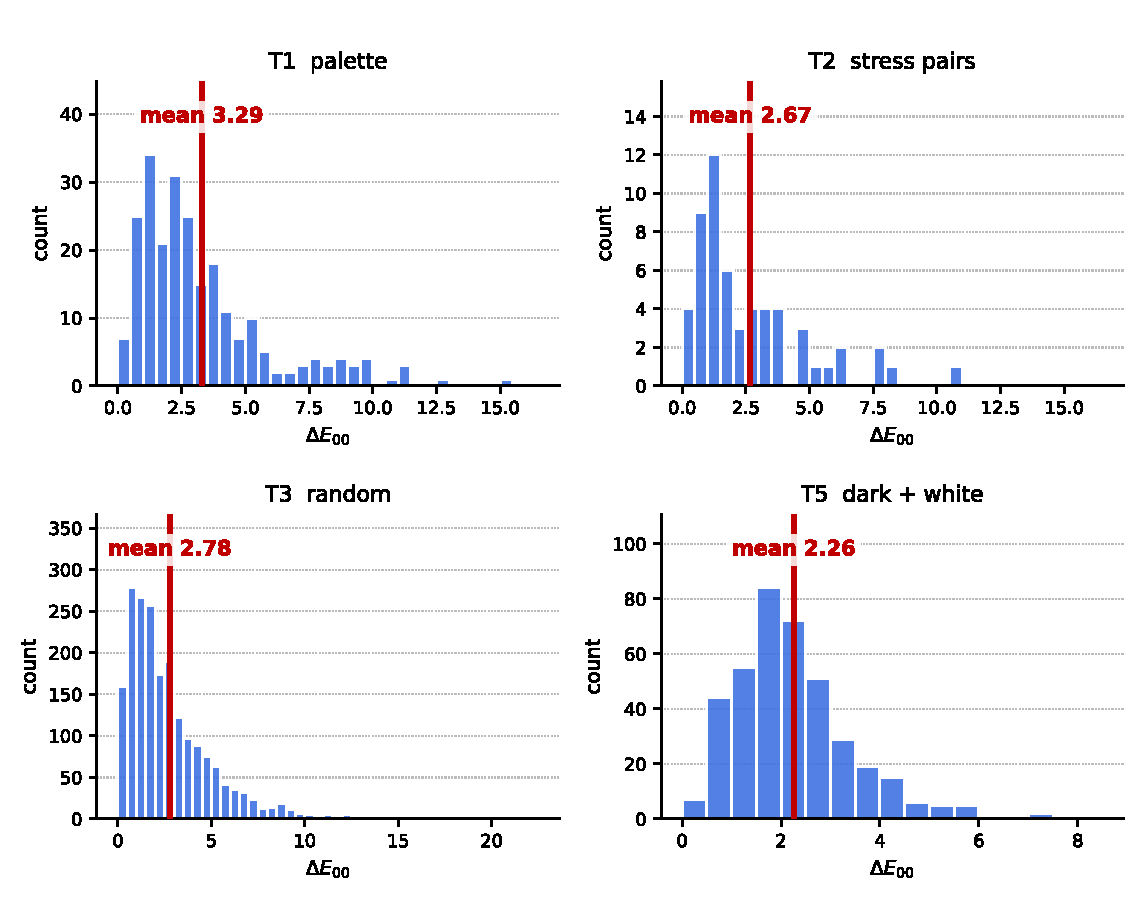
\includegraphics[width=0.72\linewidth]{fig4-error-dist.pdf}
\caption{PBM 相对 Mixbox~2.0 在 T1、T2、T3（seed 20260808，$n=2000$）与 T5 上的 $\Delta E_{00}$ 直方图（组距 0.5；红线为均值）。}
\label{fig:errhist}
\end{figure}

由此得到三点观察。第一，留出均值与拟合抽样相差至多 0.09 $\Delta E_{00}$（T3 切片 2.789 对 2.759），独立抽样（2.719 与 2.852）位于同一区间。在该协议下未发现过拟合证据。第二，留出最大值（19.4--23.8）出现在"大变明度差叠加色相对立"的随机对上；该族是大误差的主要来源（\cref{sec:errors}）。第三，深色加白修复具有泛化性：T5-留出为 2.377，仅比样本内 T5 均值高 0.12，而 RGB 插值（7.61）与原始 K--M（9.52）仍停留在样本内水平。

在 T5E（240 个样本）上，PBM 的均值为 2.441、最大值为 9.5、95 分位为 8.08，位于设计目标之内。$\varphi$ 映射的两次应用都改善了各自针对的颜色对：关闭核心映射使 T5E 均值从 2.441 升到 2.872，关闭幂律目标中的映射使其升到 2.881。

\subsection{消融}
\label{sec:ablation}

\Cref{tab:ablation} 在参考实现中逐项关闭组件。所有变体都由算法源码的文本替换生成，并已验证确实改变了被执行的代码；替换目标缺失时工具会报错。

\begin{table}[t]
\centering
\footnotesize
\setlength{\tabcolsep}{2.5pt}
\caption{消融研究（$\Delta E_{00}$ 均值 / 最大值）。T3 为 seed 20260808 的完整抽样（$n=2000$）。}
\label{tab:ablation}
\begin{tabular}{lccccc}
\toprule
配置 & T1 & T2 & T3 & T5 & tail \\
\midrule
PBM（完整） & \textbf{3.286 / 15.0} & \textbf{2.667 / 10.7} & \textbf{2.777 / 19.4} & \textbf{2.258 / 7.3} & \textbf{1.678 / 8.0} \\
$-$ 跨通道矩阵 $\Mthree$ & 3.674 / 23.8 & 3.534 / 14.9 & 3.218 / 25.6 & 2.259 / 7.3 & 1.678 / 8.0 \\
$-$ 互吸收 $\beta$ & 3.409 / 12.9 & 2.603 / 10.2 & 2.904 / 19.4 & 2.262 / 7.3 & 1.678 / 8.0 \\
$-$ 通道耦合 & 3.797 / 15.0 & 2.978 / 10.7 & 3.857 / 30.9 & 8.834 / 19.7 & 4.670 / 19.7 \\
$-$ 方向响应 & 3.491 / 15.0 & 2.741 / 10.7 & 2.969 / 24.2 & 4.739 / 15.2 & 3.429 / 12.4 \\
$-$ 谐波修正（$\hat{\gamma}$） & 3.649 / 15.3 & 3.543 / 13.5 & 2.890 / 20.0 & 2.258 / 7.3 & 1.678 / 8.0 \\
$-$ 幂律修复（$g\equiv0$） & 3.700 / 15.0 & 3.091 / 10.7 & 3.248 / 20.4 & 9.823 / 23.8 & 8.448 / 24.0 \\
幂律全接管（$g\equiv1$） & 4.785 / 25.2 & 5.237 / 24.4 & 2.967 / 26.1 & 2.248 / 7.3 & 1.654 / 8.0 \\
\bottomrule
\end{tabular}
\end{table}

在深色加白套件上，幂律修复与通道耦合仍是最强的两个贡献项：去掉修复后 T5 从 2.258 升至 9.823，去掉耦合后升至 8.834。耦合在主套件上也是最强的单项（T3 从 2.777 升至 3.857）。跨通道矩阵在主套件上次之（T1 从 3.286 升至 3.674；T2 从 2.667 升至 3.534），在修复主导的 T5 上中性。方向响应在 T5（4.739）与尾端（3.429）上重要。互吸收影响小而混杂：去掉后 T2 变好（2.603）而 T1 变差（3.409），故保留。谐波修正改善全部三个主套件（T1 3.649→3.286；T2 3.543→2.667；T3 2.890→2.777），现为单调有益的组件。强制幂律目标全接管会恶化主套件（T1 4.785、T2 5.237），故门控的区域选择是必要的。

\subsection{误差结构}
\label{sec:errors}

最大误差集中在"大变明度差叠加色相对立"的颜色对上。T1 最差对为近黑 $\#141417$ 与橙 $\#FF7A2A$ 在 $\alpha=0.25$ 处（$\Delta E_{00}=15.02$）；T2 最差对为黄 $\#FFD61A$ 与群青 $\#2E5EFF$ 在 $\alpha=0.75$ 处（10.70）；T3 最差对为浅绿灰 $\#C8D098$ 与蓝紫 $\#3A45E6$ 在 $\alpha\approx0.32$ 处（19.43）。这些混合物中，参考的七维潜空间产生逐通道独立形式无法表示的跨通道关联。在 $\alpha\in[0.05,0.95]$ 上，八个锚点对的平均 $\Delta E_{00}$ 分别为 2.85（黄 $\times$ 深蓝 $\#FFC400+\#000F3D$）、3.16（黄 $\times$ 近边界 $\#FFC400+\#000724$）、5.20（红 $\times$ 绿 $\#A30000+\#00B359$）、7.04（红 $\times$ 青 $\#A30000+\#00D5C0$）、1.79（品红 $\times$ 绿 $\#E33BA8+\#00B359$）、3.80（橙 $\times$ 蓝 $\#FF7A1A+\#2E5EFF$）、9.73（橙 $\times$ 深蓝 $\#FF7A1A+\#001B75$）、5.07（红 $\times$ 深蓝 $\#A30000+\#001B75$）；去掉谐波修正后误差显著增大（\cref{tab:ablation}）。

在 T5 上，最差的固定色对是深紫 $\#080248$ 与白在 $\alpha=0.4$ 处（$\Delta E_{00}=7.3$），随机深色的最坏情况同为 7.3。T5 中的两个近黑红（$\#280501$ 与 $\#250903$）在带范围门时于 $\alpha\in[0.1,0.9]$ 上测得均值 1.80 / 2.31、最大值 2.11 / 2.66；关闭该门会把这些值抬到 16.06 / 13.81 与 18.74 / 16.45。\Cref{fig:white,fig:worst} 给出深色加白的轨迹与最差对。

\begin{figure}[t]
\centering
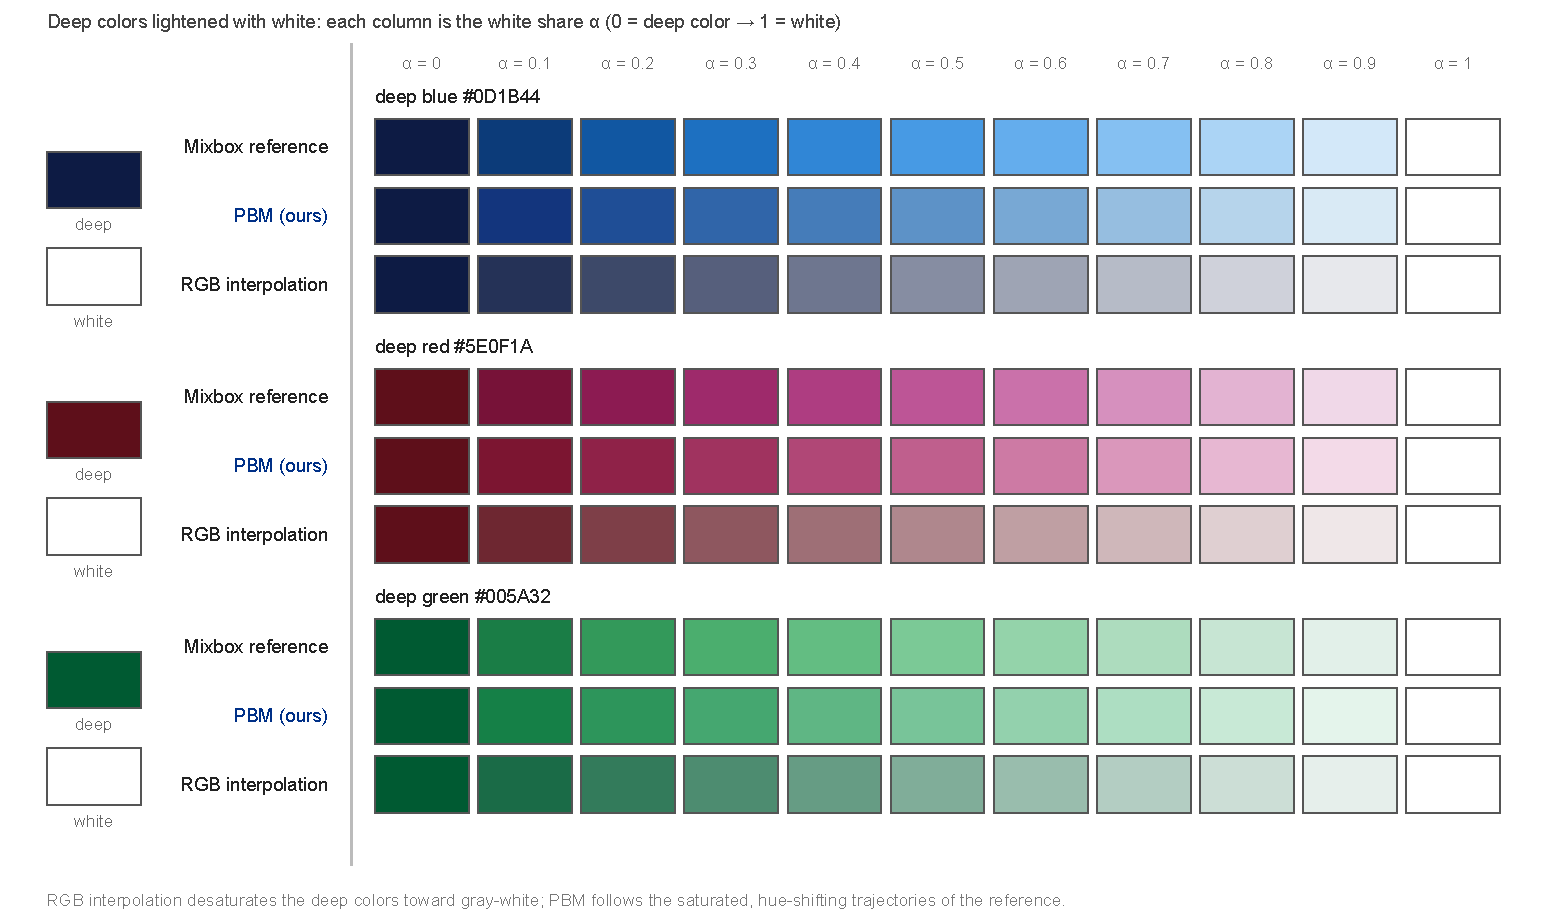
\includegraphics[width=\linewidth]{fig7-mixing-white.pdf}
\caption{深色加白。每列为白色占比 $\alpha$（$0$ = 深色，$1$ = 白）。RGB 插值朝灰白去饱和；PBM 跟随参考的有色度、有色相偏移的轨迹。}
\label{fig:white}
\end{figure}

\begin{figure}[t]
\centering
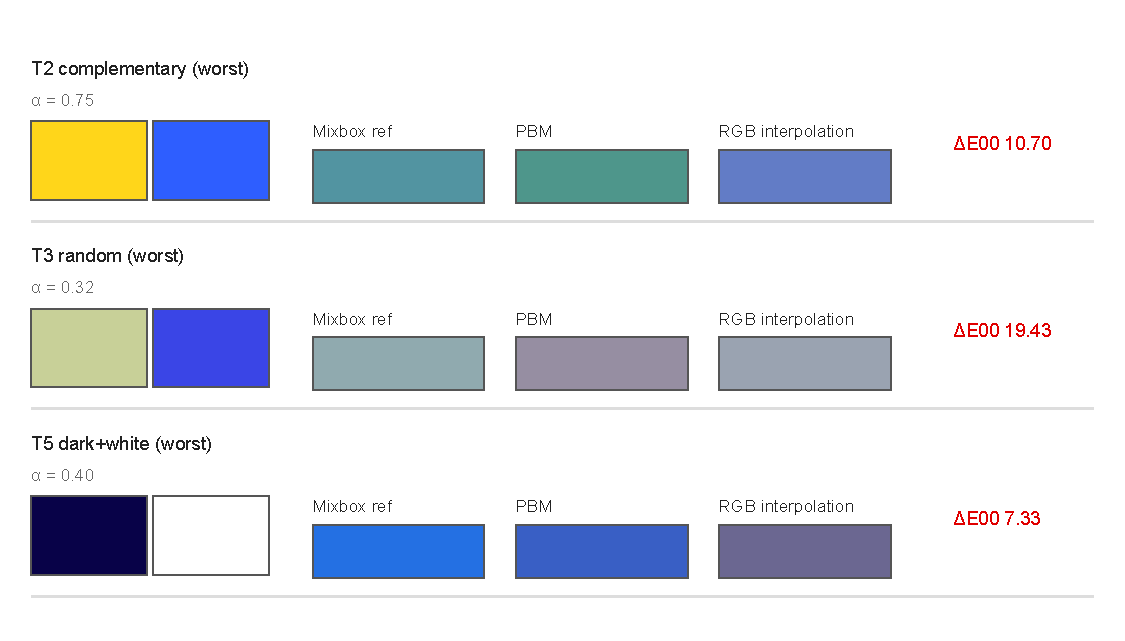
\includegraphics[width=0.82\linewidth]{fig5-worst-pairs.pdf}
\caption{T2 互补、T3 随机与 T5 深色加白套件的最差对：输入、Mixbox 参考输出、PBM 输出、RGB 插值输出，以及 $\Delta E_{00}$。}
\label{fig:worst}
\end{figure}

\subsection{连续性与交换对称}
\label{sec:continuity}

连续性探针对 4000 个随机对的每个输入通道施加 $\pm1/255$ 扰动、对比例施加 $+0.004$，记录输出的最大 $\Delta E_{00}$ 变化。最大单步变化为 1.388，超过 1.53 的次数为零。色度衰减对该结果必要：当 $\mathrm{cSat}\equiv1$ 时，同一探针测得 2.531 与 14 次超阈，原因是比值特征在消色轴附近梯度很大。\Cref{fig:continuity} 给出一个深蓝/白混合的响应。

交换对称在 5000 个随机对（seed 20260808）上测得。$F(\cb,\ct,\alpha)$ 与 $F(\ct,\cb,1-\alpha)$ 的最大 RGB 差为 $6.7\times10^{-16}$，即两分支乘法次序不同带来的浮点舍入。

\begin{figure}[t]
\centering
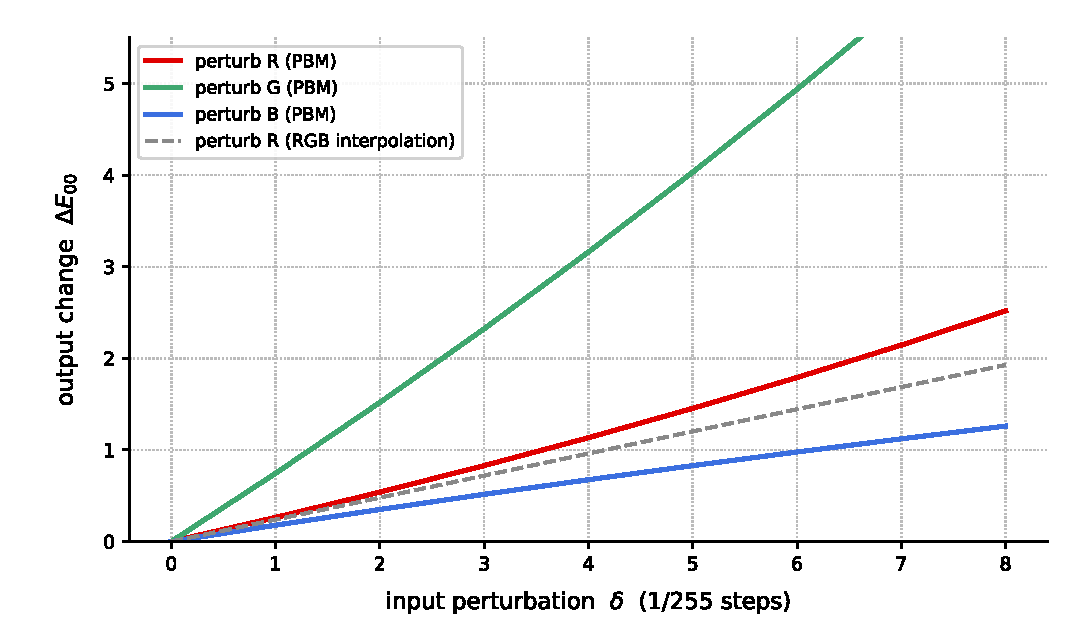
\includegraphics[width=0.72\linewidth]{fig6-continuity.pdf}
\caption{邻域连续性：输出变化 $\Delta E_{00}$ 随输入扰动的变化（对深蓝 $\#0D1B44$ 的每个通道以 1/255 步进，与白在 $\alpha=0.5$ 混合）；虚线为 RGB 插值的响应。}
\label{fig:continuity}
\end{figure}

\subsection{运行时间}
\label{sec:runtime}

\Cref{tab:runtime} 报告在 Windows~11、AMD Ryzen~5 5600X 上使用 Node.js 26.13.1 测得的单次混色时间。全部模型都在宿主 V8 上下文中加载：同一段代码若在 \texttt{node:vm} 沙箱内运行，初等函数调用（\texttt{Math.sqrt}、\texttt{Math.pow}）会被放大一到两个数量级——实测 PBM 为 $8.9\times$、参考为 $8.7\times$——从而扭曲与纯算术基准的对比。PBM、Mixbox 与 RGB 插值使用 $10^{5}$ 个确定性对、预热后九次重复取最好值；光谱 K--M 路径使用 50 对子集，因为迭代反解主导其运行时间。绝对时间依赖于机器与实现；表中比值在同一环境中测得，用于支持接口论证，而不是一般性的性能声明。

\begin{table}[t]
\centering
\small
\caption{单次混色的运行时间（预热后九次重复取最好值）。最后一列为相对 PBM 的时间比。}
\label{tab:runtime}
\begin{tabular}{llrrr}
\toprule
模型 & 路径 & ns/op & ops/s & 相对时间 \\
\midrule
PBM & 解析浮点运算 & 226 & 4{,}431{,}819 & 1.00 \\
Mixbox 2.0 & $256^{3}$ 查找表 & 166 & 6{,}021{,}376 & 0.73 \\
RGB 插值 & 线性混合 & 16 & 63{,}572{,}791 & 0.070 \\
K--M 光谱，直接 & 逐波长 K/S $+$ D65$\times$CMF & 1{,}195 & 836{,}820 & 5.3 \\
K--M 光谱，RGB 输入 & 迭代 unmix $+$ 光谱混合 & 22{,}400{,}000 & 45 & $9.9\times10^{4}$ \\
\bottomrule
\end{tabular}
\end{table}

PBM 的单次成本约为 0.23 $\mu$s，是参考查找表的 1.4 倍、线性混合的 14 倍。光谱 K--M 前向管线本身并不慢：已知颜料光谱时，逐波长积分约需 1.2 $\mu$s，约为 PBM 的 5 倍。障碍在接口：混合两个任意 RGB 颜色需要先把每个颜色反解为颜料浓度，这一迭代优化约需 22 ms，约为 PBM 的 $10^{5}$ 倍。因此 PBM 的优势不是原始速度，而是不需要光谱表示、反解或数兆字节的表。交互绘画中混色按笔触或操作应用，而不是按渲染像素；逐像素渲染时两种模型都会向量化或在 GPU 上实现，此时解析形式更易移植。谐波修正中不含三角函数与对数求值，也使其更易于向量化。

\subsection{相对独立合成光谱世界的验证}
\label{sec:synthetic}

上一节的评估把 PBM 与参考对比。本节改用由合成颜料光谱计算的真值交叉验证，这些光谱未参与 PBM 的拟合。

\paragraph{数据集.}
数据集包含 29 个颜料：覆盖色相环与中性阶的 24 个功能色相，以及用于深色加白套件的 5 个深色派生。每个颜料在 380--750 nm 的 10 nm 网格（38 个采样）上以独立的吸收与散射系数表示：
\begin{equation}
K(\lambda)=\kappa_{\mathrm{base}}+\sum_{i}A_{i}e^{-((\lambda-\mu_{i})/\sigma_{i})^{2}}
+\sum_{j}\frac{B_{j}}{1+e^{\pm((\lambda-\lambda_{j})/w_{j})}},
\qquad S(\lambda)=S_{\mathrm{base}}.
\label{eq:synthetic}
\end{equation}
带位置由第一性原理颜料化学固定（黄/橙/红族的蓝—绿陡吸收边、蓝/绿族的红侧上升边、品红的绿区带、以及过渡金属或有机特征带），幅度、宽度、基底与散射由坐标下降标定到公开的 BabelColor X-Rite ColorChecker Classic Avg30 光谱 \cite{pascale2012}（拟合 $\Delta E_{00}\le1.2$，多数色卡 $\le0.2$）。这些色卡是配方色卡光谱而非纯颜料厚涂光谱；K--M 方程对任意反射率光谱封闭，且色卡面向 RGB 显示设计，故无需显示标定。合成世界是近似，不是实测颜料。

\paragraph{管线与套件.}
前向管线分别叠加 $K$ 与 $S$，逐波长求 \cref{eq:km}，在 10 nm 网格上对 D65 与 CIE 1931 $2^{\circ}$ 观察者积分，再转为 sRGB（截断并标记色域外样本）。所有被比较模型的输入都是纯颜料的渲染 sRGB 颜色，从而避开"某些颜色无法由颜料混出"的问题。六个套件对应 T 套件结构：P1（24 色相调色板全部 828 对）、P2（9 个压力对）、P3（2000 个随机颜料对，新 seed 20260813）、P5（15 个深色颜料 $\times$ 白）、P5-buff（同一深色集 $\times$ 米色）、P5E（双侧尾端网格）。色域外样本被截断并计数。

\Cref{tab:synthetic} 报告结果，\cref{fig:physical} 展示三个代表颜色对。

\begin{table}[t]
\centering
\footnotesize
\setlength{\tabcolsep}{3pt}
\caption{相对合成光谱参考的 $\Delta E_{00}$（均值 / 最大值；随机集均值的 bootstrap 95\% 区间见注；色域外样本截断并计数）。}
\label{tab:synthetic}
\begin{tabular}{lcccccc}
\toprule
模型 & P1 & P2 & P3 & P5 & P5-buff & P5E \\
 & {\scriptsize$n{=}828$, 域外 6} & {\scriptsize$n{=}27$} & {\scriptsize$n{=}2000$, 域外 35} & {\scriptsize$n{=}135$} & {\scriptsize$n{=}135$, 域外 2} & {\scriptsize$n{=}150$, 域外 6} \\
\midrule
PBM & 6.70 / 36.3 & 13.38 / 29.7 & 5.60 / 35.9 & 8.44 / 22.3 & 4.99 / 17.1 & 3.40 / 13.9 \\
Mixbox 2.0 & 6.46 / 31.5 & 12.71 / 24.9 & 5.10 / 30.2 & 8.86 / 25.0 & 4.56 / 18.9 & 3.39 / 20.9 \\
RGB 插值 & 6.14 / 29.5 & 11.25 / 20.4 & 4.89 / 25.4 & 8.24 / 27.0 & 5.95 / 15.8 & 3.88 / 26.9 \\
K--M 显示值 & 5.55 / 30.5 & 8.82 / 16.6 & 4.38 / 30.5 & 12.13 / 30.8 & 4.95 / 18.1 & 4.25 / 28.2 \\
\bottomrule
\end{tabular}

\smallskip
{\scriptsize Bootstrap 95\% 置信区间（均值）：PBM P1 [6.320, 7.045]、P3 [5.390, 5.822]、P5 [7.610, 9.258]；Mixbox P1 [6.080, 6.808]、P3 [4.884, 5.333]、P5 [7.964, 9.786]。}
\end{table}

\begin{figure}[t]
\centering
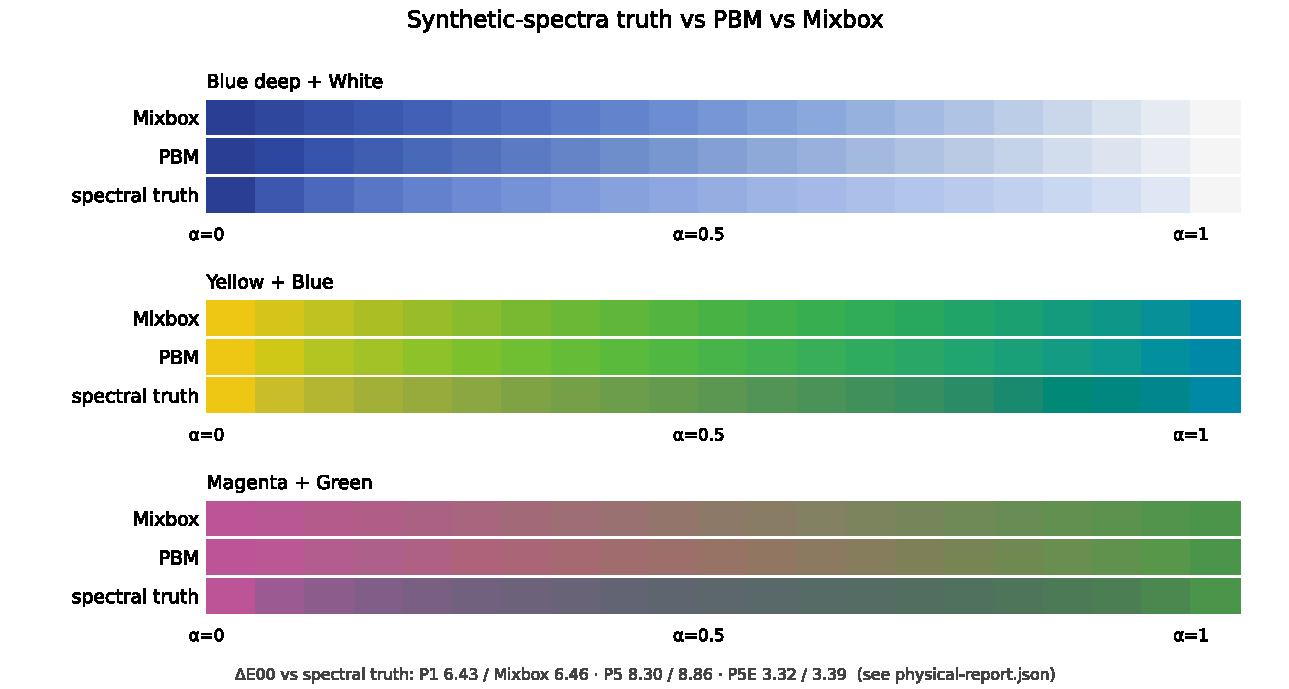
\includegraphics[width=0.88\linewidth]{fig8-physical.pdf}
\caption{合成光谱真值 versus PBM 与 Mixbox：三个代表颜料对（深蓝 $\times$ 白、黄 $\times$ 蓝、品红 $\times$ 绿）在 $\alpha=0$--$1$ 上（21 步）。}
\label{fig:physical}
\end{figure}

由此得到三点观察。第一，PBM 与参考在该世界上相当：各套件均值差 $\mathrm{PBM}-\mathrm{Mixbox}$ 在 $-0.42$（P5）到 $+0.67$（P2）之间，且每对 bootstrap 区间重叠。两者都未在该世界上训练，因此这种平价是 PBM 的精度并非拟合参考输出所致伪影的证据。PBM 在 P5 与 P5E 上更接近真值，参考在 P1、P2、P3、P5-buff 上更接近；本文未检验这些差异的显著性。第二，色相轨迹一致：\cref{tab:hue} 报告有色度样本（$C^{\ast}>10$）的平均与中位绝对色相差。PBM 的平均色相误差在六个套件中的三个（P5、P5-buff、P5E）更低，其余相差在 $2^{\circ}$ 以内。第三，各套件剩余平均误差（3.40--13.38 $\Delta E_{00}$）是结构性的：合成世界按光谱 K--M 混色，而 Mixbox 在训练的潜空间多项式上混色。

\begin{table}[t]
\centering
\small
\caption{与合成光谱真值的色相一致：有色度样本（$C^{\ast}>10$）上平均与中位绝对色相差（度）。}
\label{tab:hue}
\begin{tabular}{lcc}
\toprule
套件 & PBM & Mixbox 2.0 \\
\midrule
P1 & 11.33 / 6.62 & 11.01 / 5.96 \\
P2 & 23.17 / 17.23 & 21.46 / 18.01 \\
P3 & 9.27 / 4.62 & 8.64 / 3.73 \\
P5 & 9.54 / 5.77 & 9.67 / 7.15 \\
P5-buff & 8.59 / 5.79 & 8.62 / 5.30 \\
P5E & 2.56 / 0.62 & 2.73 / 0.74 \\
\bottomrule
\end{tabular}
\end{table}

\paragraph{该实验确立与不确立什么.}
实验支撑两点主张：(i) PBM 的精度不是对参考输出过拟合的伪影，因为它在独立合成光谱世界上与参考相当；(ii) 定性行为族——黄 $\times$ 蓝得绿、互补对得浑浊色、深 $+$ 白保持色相——在两常数光谱 K--M 混色下同样成立。它并不确立 PBM 能预测真实颜料的厚涂混色，也不确立它比参考更接近真实颜料。合成世界本身是近似，PBM 与真实颜料的关系被"参考与真实颜料的关系"加上"PBM 相对参考的实测偏差"共同界定。

\subsection{有效性威胁}
\label{sec:threats}

\paragraph{对参考的依赖.}
PBM 拟合自 Mixbox~2.0。若参考改变，常数必须按 \cref{sec:estimation} 的流程重新估计。实测精度是相对该参考的，并不界定对实测颜料样品的误差。

\paragraph{合成世界.}
交叉验证使用两常数 K--M 混合标定到 ColorChecker 色卡的合成光谱。两常数近似与色卡标定都限制了解释；合成世界不能替代实测颜料光谱。

\paragraph{度量.}
本文使用等权 CIEDE2000。其他色差公式或观察者/光源选择可能改变个别颜色对的排序并影响报告的均值。

\paragraph{抽样.}
固定套件为样本内；只有随机集给出置信区间。置信区间覆盖均值的抽样波动，不覆盖模型选择或实现不确定性。

\paragraph{范围.}
模型定义于 sRGB 显示值空间中不透明、均匀混合的颜色。它不建模分层、罩染、透明度、纹理或光谱输出。
